\chapter{Atomo di Elio}
L'atomo (neutro) di elio (He) è costituito da un nucleo di carica \( Ze \) con \( Z = 2 \) e due elettroni. 
Sia \( M_N \) la massa del nucleo e si scelga come sistema di riferimento quello esposto in figura dove i vettori posizione dei due elettroni e del nucleo sono indicati da \( \vec{r}_{e,1}, \vec{r}_{e,2}, \vec{R}_N \) rispettivamente. 
Si definisca inoltre \( \vec{r}_{e,1-2} = \vec{r}_{e,2} - \vec{r}_{e,1} \) la posizione relativa dei due elettroni. 

\begin{figure}[htbp]
    \centering
    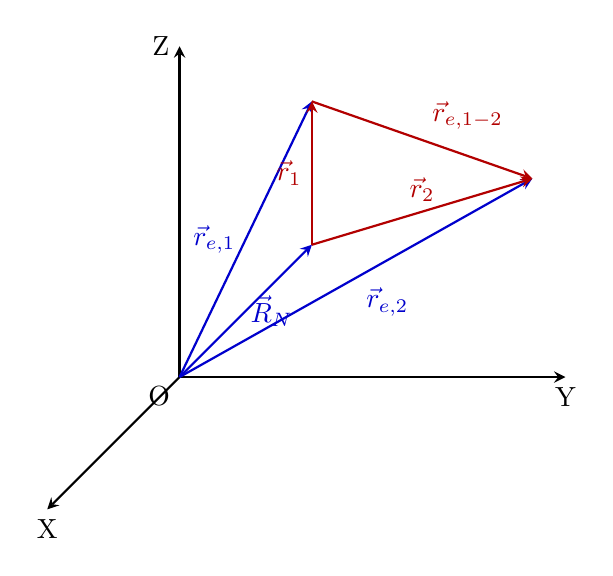
\begin{tikzpicture}[>=stealth, scale=1.4]
        % Assi cartesiani (SR LAB)
        \draw[->, thick] (0,0) -- (0,3) node[left] {Z};
        \draw[->, thick] (0,0) -- (3.5,0) node[below] {Y};
        \draw[->, thick] (0,0) -- (-1.2,-1.2) node[below] {X};
        \node[below left] at (0,0) {O};

        % Coordinate
        \coordinate (N) at (1.2, 1.2);   % Nucleo
        \coordinate (E1) at (1.2, 2.5); % Elettrone 1
        \coordinate (E2) at (3.2, 1.8); % Elettrone 2

        % Vettori posizione dal SR LAB (in blu)
        \draw[->, thick, blue!80!black] (0,0) -- (N) node[midway, right, xshift=-2pt] {\( \vec{R}_N \)};
        \draw[->, thick, blue!80!black] (0,0) -- (E1) node[midway, left] {\( \vec{r}_{e,1} \)};
        \draw[->, thick, blue!80!black] (0,0) -- (E2) node[midway, below right] {\( \vec{r}_{e,2} \)};

        % Vettori relativi (in rosso)
        \draw[->, thick, red!70!black] (N) -- (E1) node[midway, left] {\( \vec{r}_1 \)};
        \draw[->, thick, red!70!black] (N) -- (E2) node[midway, above] {\( \vec{r}_2 \)};
        \draw[->, thick, red!70!black] (E1) -- (E2) node[midway, above right] {\( \vec{r}_{e,1-2} \)};
    \end{tikzpicture}
    \caption{Sistema di riferimento e coordinate vettoriali per l'atomo di elio.}
    \label{fig:atomo_elio_vettori}
\end{figure}
L'operatore Hamiltoniano \( H \) per l'atomo di He è fornito dalla seguente espressione:
\begin{equation}
    H = -\frac{\hbar^2}{2M_N} \nabla_{\vec{R}_N}^2 - \frac{\hbar^2}{2m_e} \nabla_{\vec{r}_{e,1}}^2 - \frac{\hbar^2}{2m_e} \nabla_{\vec{r}_{e,2}}^2 - \frac{Ze^2}{4\pi\epsilon_0 r_1} - \frac{Ze^2}{4\pi\epsilon_0 r_2} + \frac{e^2}{4\pi\epsilon_0 r_{e,1-2}} + \Delta H_{SF}
\end{equation}

Dove \( \Delta H_{SF} \) indica il contributo di correzione di struttura fine.

Per risolvere l'equazione di Schrödinger associata è conveniente fin da subito passare a un sistema di riferimento in cui la simmetria del problema possa semplificare i conti. 
Questo è il caso del sistema di riferimento del centro di massa (CM) individuato dal vettore posizione \( \vec{R}_{CM} \) e la cui massa ridotta è data da \( \mu = \frac{m_e M_N}{m_e + 2M_N} \).
Essendo il nucleo con massa \( M_N \gg m_e \), in prima approssimazione si può assumere che \( \vec{R}_{CM} \approx \vec{R}_N \). Inoltre, si consideri per semplicità il nucleo fermo.

Nel sistema di riferimento del centro di massa l'atomo di He sarà perciò descritto da:

\begin{equation}
    H = -\frac{\hbar^2}{2\mu} \nabla_{r_1}^2 - \frac{\hbar^2}{2\mu} \nabla_{r_2}^2 - \frac{Ze^2}{4\pi\epsilon_0 r_1} - \frac{Ze^2}{4\pi\epsilon_0 r_2} + \frac{e^2}{4\pi\epsilon_0 r_{12}} + \Delta H_{SF} - \frac{\hbar^2}{M_N} \vec{\nabla}_{r_1} \cdot \vec{\nabla}_{r_2}
\end{equation}

dove il termine \( -\frac{\hbar^2}{M_N} \vec{\nabla}_{r_1} \cdot \vec{\nabla}_{r_2} \) è detto \textbf{termine di polarizzazione di massa} ed emerge a seguito del cambio di coordinate. Dato che \( M_N \gg m_e \), esso contribuisce in modo poco significativo e può esser trascurato (di norma è incluso solo per correzioni di ordine superiore).

Le autofunzioni associate a \( H \):
\begin{equation}
    \Psi_E(\vec{r}_1, \vec{r}_2, \vec{R}_{CM}, s_1, s_2)
\end{equation}

Per stimare lo spettro in energia di He, la prima ipotesi è \( H \approx H^{(0)} \). Si tratta di un'ipotesi perturbativa in cui si assume che gli elettroni non interagiscano tra loro. L'Hamiltoniana imperturbata si scrive come somma di due Hamiltoniane idrogenoidi indipendenti:
\begin{equation}
    H^{(0)} = \underbrace{(T_1 + V_{N-1})}_{H_1} + \underbrace{(T_2 + V_{N-2})}_{H_2}
\end{equation}

\subsubsection{Proprietà autofunzioni}
Per l'Hamiltoniana imperturbata è possibile separare per variabili le autofunzioni:
\begin{equation}
    \Psi_E(\vec{r}_1, \vec{r}_2, \vec{R}_{CM}, s_1, s_2)= \Psi^{(0)}_E(\vec{r}_1, \vec{r}_2)\chi(s_1,s_2)   \Phi(\vec{R}_{CM})
\end{equation}
Dove possiamo trascurare l'ultimo termine considerando il nucleo fermo.

La funzione d'onda totale \(\Psi_E (\vec{r}_1, \vec{r}_2, \vec{R}_{CM}, s_1, s_2)\) deve essere antisimmetrica per elettroni indistinguibili.

\textbf{Proprietà di} \(\Psi_E^{(0)}(\vec{r}_1, \vec{r}_2)\):
L'Hamiltoniana imperturbata \(H^{(0)}\) è invariante per lo scambio dei due elettroni (trattandosi di Fermioni).
Sia \(\lambda = \pm 1\) l'autovalore associato all'operatore di scambio \(P \) (parità). Allora si dovrà verificare che:
\begin{equation}
    \begin{cases}
        \Psi_E^{(0)}(\vec{r}_2, \vec{r}_1) = \lambda \Psi_E^{(0)}(\vec{r}_1, \vec{r}_2) \\
        \lambda^2 = 1
    \end{cases}
\end{equation}

Ovvero:
\begin{equation}
    \Psi_E^{(0)}(\vec{r}_1, \vec{r}_2) = -\Psi_E^{(0)}(\vec{r}_2, \vec{r}_1) \quad \text{oppure} \quad \Psi_E^{(0)}(\vec{r}_1, \vec{r}_2) = \Psi_E^{(0)}(\vec{r}_2, \vec{r}_1)
\end{equation}

Dunque la parte spaziale può risultare antisimmetrica o simmetrica. Per il principio di esclusione di Pauli, la funzione d'onda totale \(\Psi_{E_{TOT}}^{(0)}\) deve essere necessariamente antisimmetrica. Per soddisfare tale condizione, occorre abbinare una parte spaziale simmetrica con una parte di \textbf{spin} antisimmetrica, e viceversa.

Dato che l'Hamiltoniana imperturbata è la somma di due contributi indipendenti \( H^{(0)} = H_1^{(0)} + H_2^{(0)} \), le variabili risultano separabili. Di conseguenza, la funzione d'onda spaziale totale \(\Psi_E^{(0)}(\vec{r}_1, \vec{r}_2)\) può essere scritta come combinazione lineare di prodotti di funzioni d'onda a singolo elettrone:
\begin{equation}
    \underbrace{H_i^{(0)} \psi_E^{(0)}(\vec{r}_i) = E_i^{(0)} \psi_E^{(0)}(\vec{r}_i)}_{\text{problema di atomo idrogenoide}} \qquad i=1,2
\end{equation}

Poiché deve valere la condizione di simmetria o antisimmetria \(\Psi_E^{(0)}(\vec{r}_1, \vec{r}_2) = \pm \Psi_E^{(0)}(\vec{r}_2, \vec{r}_1)\), la funzione d'onda viene costruita come:
\begin{equation}
    \Psi_E^{(0)}(\vec{r}_1, \vec{r}_2) = \mathcal{K} \left( \psi_{n_1, \ell_1, m_{\ell_1}}^{(0)}(\vec{r}_1) \psi_{n_2, \ell_2, m_{\ell_2}}^{(0)}(\vec{r}_2) \pm \psi_{n_1, \ell_1, m_{\ell_1}}^{(0)}(\vec{r}_2) \psi_{n_2, \ell_2, m_{\ell_2}}^{(0)}(\vec{r}_1) \right)
\end{equation}
dove \(\mathcal{K}\) rappresenta la \textbf{costante di normalizzazione}.

Definiamo in modo contratto tali stati con il simbolo \(\Psi_{E, \pm}^{(0)}(\vec{r}_1, \vec{r}_2)\):
\begin{itemize}
    \item \(\Psi_{E, +}^{(0)}\): combinazione \textbf{simmetrica} rispetto allo scambio \(\vec{r}_1 \leftrightarrow \vec{r}_2\);
    \item \(\Psi_{E, -}^{(0)}\): combinazione \textbf{antisimmetrica} rispetto allo scambio \(\vec{r}_1 \leftrightarrow \vec{r}_2\).
\end{itemize}

\subsubsection{Autofunzioni di Spin}Consideriamo la funzione d'onda di spin complessiva \(\chi(1, 2)\). Per ogni elettrone (\(i=1,2\)), definiamo l'operatore di spin di singola particella \(\vec{S}_i\) tramite le sue componenti:
\begin{equation}
    \vec{S}_i = (S_{ix}, S_{iy}, S_{iz})
\end{equation}

L'operatore di spin totale del sistema è la combinazione (somma) dei contributi di ogni singolo fermione:
\begin{equation}
    \vec{S} = \vec{S}_1 + \vec{S}_2
\end{equation}

L'operatore di modulo quadro dello spin totale assume la forma:
\begin{equation}
    S^2 = S_1^2 + S_2^2 + 2\vec{S}_1 \cdot \vec{S}_2
\end{equation}

Definiamo inoltre la componente lungo l'asse \(z\) dell'operatore totale \(\vec{S} = (S_x, S_y, S_z)\) come:
\begin{equation}
    S_z = S_{1z} + S_{2z}
\end{equation}

L'insieme \(\{\chi(1, 2)\}\) rappresenta il set di autofunzioni comuni agli operatori \(S^2\) e \(S_z\). Poiché \(\vec{S}\) descrive la somma di due momenti angolari, esso segue rigorosamente le regole di composizione del momento angolare.

Siano \(\alpha = \ket{\uparrow}\) e \(\beta = \ket{\downarrow}\) gli autostati di spin del singolo elettrone. Gli autovalori (autofunzioni di \(S^2\)) sono legati al numero quantico di spin \(s\), che per l'elettrone assume il valore \(s=1/2\).

All'operatore di spin totale \(\vec{S}\) associamo il numero quantico di spin totale \(s\). Secondo le regole di composizione del momento angolare, i valori permessi per \(s\) sono vincolati dalla relazione:

\begin{importantbox}
    \begin{equation}
        |s_1 - s_2| \le s \le s_1 + s_2 
    \end{equation}
\end{importantbox}

Considerando che per ogni elettrone \(s_i = 1/2\), nel caso di un sistema a due elettroni (come l'atomo di Elio), il numero quantico totale può assumere i valori \(s = 0, 1\). Allo spin totale \(\vec{S} = \vec{S}_1 + \vec{S}_2\) si associa il numero quantico magnetico \(m_s\), il quale può assumere \(2s+1\) valori compresi nell'intervallo:
\begin{equation}
    m_s = -s, -s+1, \dots, s
\end{equation}

Per indicizzare correttamente l'autofunzione di spin complessiva \(\chi(1,2)\), utilizziamo la base formata dai numeri quantici \(s\) e \(m_s\):
\begin{equation}
    \chi(1,2) = \chi_{s, m_s}
\end{equation}

Per rispettare il \textbf{principio di Pauli}, il set di autofunzioni \(\{\chi(1,2)\}\) deve possedere una "parità definita" rispetto allo scambio delle particelle. Ciò significa che le funzioni d'onda devono essere intrinsecamente \textbf{simmetriche} o \textbf{antisimmetriche}.
Soddisfano a tali requisiti di parità definita e di essere autofunzioni di \(S^2\) e \(S_z\) le seguenti combinazioni lineari degli autostati di singola particella:

\begin{equation}
    \chi(1,2) \longrightarrow
    \begin{cases}
        \chi_1(1,2) = \alpha(1)\alpha(2) = \ket{\uparrow\uparrow} \\[1.5ex]
        \chi_+(1,2) = \displaystyle\frac{\alpha(1)\beta(2) + \alpha(2)\beta(1)}{\sqrt{2}} = \frac{\ket{\uparrow\downarrow} + \ket{\downarrow\uparrow}}{\sqrt{2}} \\[2.5ex]
        \chi_-(1,2) = \displaystyle\frac{\alpha(1)\beta(2) - \alpha(2)\beta(1)}{\sqrt{2}} = \frac{\ket{\uparrow\downarrow} - \ket{\downarrow\uparrow}}{\sqrt{2}} \\[2.5ex]
        \chi_4(1,2) = \beta(1)\beta(2) = \ket{\downarrow\downarrow}
    \end{cases}
\end{equation}

Si osserva che gli stati \(\chi_1, \chi_+\) e \(\chi_4\) formano il \textbf{tripletto} (stati simmetrici con numero quantico di spin totale \(s=1\)), mentre lo stato \(\chi_-\) è il \textbf{singoletto} (stato antisimmetrico con \(s=0\)).

\begin{attention}
    Si verifica analiticamente che:
    \begin{equation}
        \chi_3(1,2) = \alpha(1)\beta(2), \qquad \chi_2(1,2) = \alpha(2)\beta(1)
    \end{equation}
    \textbf{non} sono autofunzioni degli operatori \(S^2\) e \(S_z\) complessivi del sistema.
\end{attention}

\begin{figure}[H]
    \centering
    \large
    \renewcommand{\arraystretch}{1.5}
    \setlength{\tabcolsep}{12pt} 
    \begin{tabular}{|c|c|c|c|c|c|}
        \hline
        \(\chi\) & \textbf{Parità} & \(s\) & \(m_s\) & \(s(s+1)\) & \(\chi_{s, m_s}\) \\ \hline
        \(\chi_-\) & Antisimmetrica & 0 & 0 & 0 & \(\chi_{0,0}\) \\ \hline
        \(\chi_1\) & Simmetrica & 1 & 1 & 2 & \(\chi_{1,1}\) \\ \hline
        \(\chi_+\) & Simmetrica & 1 & 0 & 2 & \(\chi_{1,0}\) \\ \hline
        \(\chi_4\) & Simmetrica & 1 & -1 & 2 & \(\chi_{1,-1}\) \\ \hline
    \end{tabular}
    \caption{Riepilogo dei numeri quantici di spin e della parità per gli stati di singoletto e di tripletto.}
    \label{fig:tabella_stati_spin_larga}
\end{figure}

Applicando l'Hamiltoniana imperturbata alla funzione d'onda totale dello stato fondamentale, otteniamo l'energia totale come somma dei singoli contributi:
\begin{equation}
    H^{(0)} \Psi_{E,\pm} \chi_{s,m_s} = E^{(0)} \Psi_{E,\pm} \chi_{s,m_s} \implies E^{(0)} = E_1^{(0)} + E_2^{(0)}
\end{equation}

Se assumiamo che l'Hamiltoniana sia separabile, \(H^{(0)} = H_1^{(0)} + H_2^{(0)}\) (dove ogni termine \(H_i^{(0)} = T_i + V_{N-i}\) rappresenta il problema indipendente per un atomo idrogenoide), l'autovalore dell'energia totale risulta:
\begin{equation}
    E^{(0)} = E_{n_1}^{(0)} + E_{n_2}^{(0)}
\end{equation}

Ricordando la formula dell'energia per i livelli di un atomo idrogenoide:
\begin{equation}
    E_n^{(0)} = -\frac{1}{2} \mu c^2 (Z\alpha)^2 \frac{1}{n^2}
\end{equation}

Possiamo riscrivere esplicitamente l'energia totale del sistema a due elettroni raccogliendo i termini comuni:
\begin{equation}
    E^{(0)} = -\frac{1}{2} \mu c^2 (Z\alpha)^2 \left( \frac{1}{n_1^2} + \frac{1}{n_2^2} \right)
\end{equation}

Per l'atomo di Elio (\(Z=2\)), nello \textbf{stato fondamentale} i due elettroni occupano il livello energetico più basso, per cui si ha \(n_1 = n_2 = 1\). Di conseguenza, l'energia imperturbata teorica equivale a due volte l'energia del livello base dell'atomo idrogenoide valutata a \(Z=2\):
\begin{equation}
    E_{\text{stato fond.}}^{(0) He} \simeq -108.8 \text{ eV}
\end{equation}

Tuttavia, questo calcolo risulta notevolmente diverso dalle evidenze sperimentali. Dal punto di vista sperimentale, infatti, l'energia misurata dello stato fondamentale è molto meno profonda:
\begin{equation}
    E_{\text{stato fond.}}^{He} \sim -78.8 \text{ eV}
\end{equation}

\lezione{8}{17/03/2026}
